\documentclass[a4paper,11pt, notitlepage]{article}

\usepackage[utf8]{inputenc}
\usepackage[T1]{fontenc}

\usepackage[top=2.5cm, bottom=3cm, left=3cm, right=3cm, headsep=14pt]{geometry}
\usepackage{graphicx}
\graphicspath{{images/}}
\usepackage[export]{adjustbox}

\usepackage{datetime}
\usepackage{float}
\usepackage{a4wide}
\usepackage[super]{nth}
\usepackage{mathtools}
\usepackage{hyperref}
\usepackage{fancyvrb}
\usepackage{booktabs}
\usepackage{multirow}
\usepackage{caption}

\usepackage{natbib}
\bibliographystyle{unsrt}


\setlength{\parskip}{0.5em}

\begin{document}

\title{
\vspace{-3cm}
Report 3 - CUDA}
\author{Nguyen Nhu Khoa - M.ICT.06.003}
\maketitle

\pagestyle{plain}
\setcounter{page}{1}

\vspace{-1cm}
\newdate{date}{31}{10}{2017}
\noindent

\section{Labwork Implementation}
Kernel:
\begin{flushleft}
\footnotesize
\begin{BVerbatim}
__global__ void grayscaleConvert2D(char* input, char* output, int imagePixelCount, int imageWidth){
    int row = threadIdx.y + blockIdx.y * blockDim.y;
    int i = row * imageWidth + threadIdx.x +blockIdx.x * blockDim.x;

    if(i < imagePixelCount){

        char g = (char) (((int) input[i * 3] + (int) input[i * 3 + 1] +
                                      (int) input[i * 3 + 2]) / 3);
        output[i * 3] =  output[i * 3 + 1] = output[i * 3 + 2] = g;
    }
}
\end{BVerbatim}
\end{flushleft}
~\\
Labwork4 function:
\begin{flushleft}
\footnotesize
\begin{BVerbatim}
void Labwork::labwork4_GPU() {
    int pixelCount = inputImage->width * inputImage->height;
    outputImage = static_cast<char *>(malloc(pixelCount * 3)); 

    char *blockSizeEnv = getenv("CUDA_BLOCK_SIZE");

    if(!blockSizeEnv){
        printf("No Environment Variable specified\n");
        printf("Please use > CUDA_BLOCK_SIZE=block_size ./labwork ...\n");
        return;
    }

    int blockSizeValue = atoi(blockSizeEnv);
    
    int gridWidth = (inputImage->width + blockSizeValue - 1)/blockSizeValue;
    int gridHeight = (inputImage->height + blockSizeValue - 1)/blockSizeValue;

    dim3 gridSize = dim3(gridWidth,gridHeight);
    dim3 blockSize = dim3(blockSizeValue,blockSizeValue);

    char *cuInput, *cuOutput;
    cudaMalloc(&cuInput, pixelCount*3*sizeof(char));
    cudaMalloc(&cuOutput, pixelCount*3*sizeof(char));
    
    cudaMemcpy(cuInput, inputImage->buffer, pixelCount*3*sizeof(char), cudaMemcpyHostToDevice);
    
    for (int j = 0; j < 100; j++) {     // let's do it 100 times, otherwise it's too fast!
        grayscaleConvert2D<<<gridSize, blockSize>>>(cuInput, cuOutput, pixelCount, inputImage->width);
    }
    cudaMemcpy(outputImage, cuOutput, pixelCount*3*sizeof(char), cudaMemcpyDeviceToHost);
    
    cudaFree(cuOutput);
    cudaFree(cuInput);   
}
\end{BVerbatim}
\end{flushleft}

\section{Speedup}
With 2D block size of 32, the program's performance does not vary too much from its 1D block counter part

\section{Other 2D block configuration}
\begin{figure}[H]
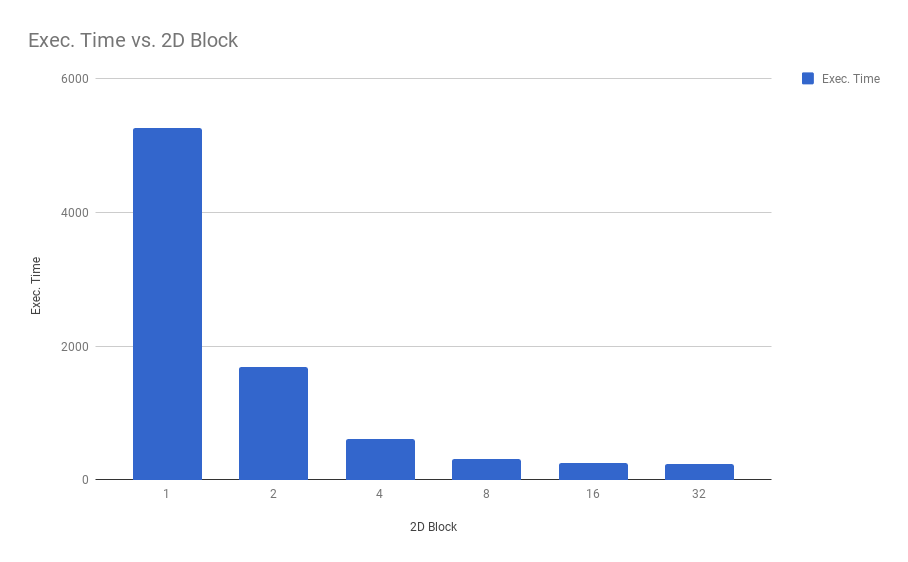
\includegraphics[width=15cm]{chart-2d.png}
\centering
\caption{2D Block Size Performance Comparison}
\end{figure}
~\\
\end{document}